\documentclass{article}

\usepackage[a4paper, total={7in, 10in}]{geometry}

\usepackage{hyperref}
\usepackage{amsmath}
\usepackage{amsfonts}
\usepackage{subcaption}
\usepackage{parskip}
\usepackage{xcolor}
\usepackage{graphicx}
\graphicspath{{../assignment/Results/Protected/}}

\title{
    AIMS Course 4: Machine Learning \\
    \large Assignment On Automatic Differentiation
}
\author{Jake Levi}
\date{November 2022}

\begin{document}
\maketitle
\section{Introduction} \label{section:intro}
We consider optimisation problems consisting of a decision variable $x$, which takes values in a set $\mathcal{X}$ (referred to as the domain of $x$), an objective function $f_0(x)$, inequality constraints $f_i(x)$ (for $i\in\{1, \hdots, m\}$), and equality constraints $h_i(x)$ (for $i\in\{1, \hdots, p\}$), which can be expressed in` the following form:
\begin{equation}
\begin{aligned}
    \underset{x \in \mathcal{X}}{\text{Minimise}} \quad & f_0(x) \\
    \text{Subject to} \quad & f_i(x) \le 0 \quad i\in\{1, \hdots, m\} \\
    & h_i(x) = 0 \quad i\in\{1, \hdots, p\}
\end{aligned} \label{eq:optimisation problem}
\end{equation}
We refer to the set of values of $x\in\mathcal{X}$ which satisfy the equality and inequality constraints as the feasible set, which is denoted by $\mathcal{F}$:
\begin{equation}
    \mathcal{F} = \{ x\in\mathcal{X}: (\forall i\in\{1, \hdots, m\}) \quad f_i(x) \le 0 \quad \text{and} \quad (\forall i\in\{1, \hdots, p\}) \quad h_i(x) = 0 \}
\end{equation}
The limit of the smallest value of $f_0(x)$ for any value of $x$ in the feasible set $\mathcal{F}$ is referred to as the optimal cost, and denoted by $p^*$:
\begin{equation}
    p^* = \underset{x\in\mathcal{F}}{\inf}\left[f_0(x)\right]
\end{equation}
When solving an optimisation problem in the form described by equation \ref{eq:optimisation problem}, it is useful to introduce the Lagrangian function \cite{boyd2004convex} (intuition for the form of the Lagrangian function is provided in appendix \ref{appendix:why lagrangian}), which is a function of the decision variable $x\in\mathcal{X}$, and also the variables $\lambda \in \mathbb{R}^m $ and $\nu\in\mathbb{R}^p$, which are referred to as the Lagrange multipliers for the inequality and equality constraints respectively:
\begin{equation}
    \mathcal{L}(x, \lambda, \nu) = f_0(x) + \sum_{i=1}^{m}[\lambda_i f_i(x)] + \sum_{i=1}^{p}[\nu_i h_i(x)] \label{eq:Lagrangian}
\end{equation}
The limit of the smallest value of the Lagrangian function for any value of $x$ in its domain $\mathcal{X}$ (not only in the feasible set $\mathcal{F}$) as a function of the Lagrange multipliers $\lambda$ and $\nu$ is referred to as the Lagrange dual function $g$:
\begin{align}
    g(\lambda, \nu) &= \underset{x\in\mathcal{X}}{\inf}\left[\mathcal{L}(x, \lambda, \nu)\right] \label{eq:dual function} \\
    &= \underset{x\in\mathcal{X}}{\inf}\left[f_0(x) + \sum_{i=1}^{m}[\lambda_i f_i(x)] + \sum_{i=1}^{p}[\nu_i h_i(x)]\right]
\end{align}
The dual function is concave with respect to $\lambda$ and $\nu$, which is equivalent to the following statements:
\begin{align}
    (\forall\lambda^{(1)},\lambda^{(2)}\in\mathbb{R}^m)(\forall\alpha\in[0, 1]) \quad g(\alpha\lambda^{(1)} + (1 - \alpha)\lambda^{(2)}, \nu) &\ge \alpha g(\lambda^{(1)}, \nu) + (1 - \alpha) g(\lambda^{(2)}, \nu) \label{eq:dual concave lambda} \\
    (\forall\nu^{(1)},\nu^{(2)}\in\mathbb{R}^p)(\forall\alpha\in[0, 1]) \quad g(\lambda, \alpha\nu^{(1)} + (1 - \alpha)\nu^{(2)}) &\ge \alpha g(\lambda, \nu^{(1)}) + (1 - \alpha) g(\lambda, \nu^{(2)})\label{eq:dual concave nu}
\end{align}
Both of these statements can be easily proved. We start by proving equation \ref{eq:dual concave lambda}, for which it is useful to define the variable $x^*\in\bar{\mathcal{X}}$ (where $\bar{\mathcal{X}}$ denotes the closure of the set $\mathcal{X}$) which satisfies the following equation, given $\alpha$, $\lambda^{(1)}$, $\lambda^{(2)}$, and $\nu$:
\begin{align}
    \underset{x\in\mathcal{X}}{\inf}\left[\mathcal{L}(x, \alpha\lambda^{(1)} + (1 - \alpha)\lambda^{(2)}, \nu)\right] &= \mathcal{L}(x^*, \alpha\lambda^{(1)} + (1 - \alpha)\lambda^{(2)}, \nu) \\
    \Rightarrow & \begin{cases}
        \underset{x\in\mathcal{X}}{\inf}\left[\mathcal{L}(x, \lambda^{(1)}, \nu)\right] \le \mathcal{L}(x^*, \lambda^{(1)}, \nu) \\
        \underset{x\in\mathcal{X}}{\inf}\left[\mathcal{L}(x, \lambda^{(2)}, \nu)\right] \le \mathcal{L}(x^*, \lambda^{(2)}, \nu)
    \end{cases} \\
    \Rightarrow \alpha \underset{x\in\mathcal{X}}{\inf}\left[\mathcal{L}(x, \lambda^{(1)}, \nu)\right] + (1 - \alpha) \underset{x\in\mathcal{X}}{\inf}\left[\mathcal{L}(x, \lambda^{(2)}, \nu)\right] &\le \alpha\mathcal{L}(x^*, \lambda^{(1)}, \nu) + (1 - \alpha)\mathcal{L}(x^*, \lambda^{(2)}, \nu) \\
    &= \mathcal{L}(x^*, \alpha\lambda^{(1)} + (1 - \alpha)\lambda^{(2)}, \nu) \label{eq:follows from Lagrangian} \\
    &= \underset{x\in\mathcal{X}}{\inf}\left[\mathcal{L}(x, \alpha\lambda^{(1)} + (1 - \alpha)\lambda^{(2)}, \nu)\right] \\
    \Rightarrow (\forall\lambda^{(1)},\lambda^{(2)}\in\mathbb{R}^m)(\forall\alpha\in[0, 1]) \quad \alpha g(\lambda^{(1)}, \nu) + (1 - \alpha) g(\lambda^{(2)}, \nu) &\le g(\alpha\lambda^{(1)} + (1 - \alpha)\lambda^{(2)}, \nu) \label{eq:follows from dual}
\end{align}
Where (\ref{eq:follows from Lagrangian}) follows from the definition of the Lagrangian function $\mathcal{L}$ in equation \ref{eq:Lagrangian} and the fact that $\alpha + (1 - \alpha) = 1$, and (\ref{eq:follows from dual}) follows from the definition of the Lagrangian dual function $g$ in equation \ref{eq:dual function}. The proof that the dual Lagrangian function is concave with respect to $\nu$ (equation \ref{eq:dual concave nu}) follows using similar reasoning.

We also note that for any $\lambda \ge 0$ (where $\ge$ is understood to apply element-wise to each element of $\lambda$) and for any $\nu$, the Lagrangian dual function $g(\lambda, \nu)$ is a lower bound for the optimal cost $p^*$. To prove this, it is useful to note that for any feasible point $\tilde{x}\in\mathcal{F}$ (which necessarily satisfies $f_i(x) \le 0$ for all $i\in\{1, \hdots, m\}$ and $h_i(x) = 0$ for all $i\in\{1, \hdots, p\}$), and for any $\lambda\ge 0$ and any $\nu$, the following inequality holds:
\begin{align}
    (\forall \tilde{x} \in \mathcal{F}, \lambda \ge 0, \nu) \quad 0 &\ge \sum_{i=1}^{m}[\lambda_i f_i(\tilde{x})] + \sum_{i=1}^{p}[\nu_i h_i(\tilde{x})] \\
    \Rightarrow (\forall \tilde{x} \in \mathcal{F}, \lambda \ge 0, \nu) \quad f_0(\tilde{x}) &\ge f_0(\tilde{x}) + \sum_{i=1}^{m}[\lambda_i f_i(\tilde{x})] + \sum_{i=1}^{p}[\nu_i h_i(\tilde{x})] \\
    &= \mathcal{L}(\tilde{x}, \lambda, \nu) \\
    &\ge \underset{x\in\mathcal{X}}{\inf}\left[\mathcal{L}(x, \lambda, \nu)\right] \\
    &= g(\lambda, \nu)
\end{align}
Since this is true for any feasible $\tilde{x}$, it is also true for the value of $\tilde{x} \in \mathcal{F}$ which minimises the objective function, $f_0(x)$:
\begin{align}
    (\forall \tilde{x} \in \mathcal{F}, \lambda \ge 0, \nu) \quad g(\lambda, \nu) &\le f_0(\tilde{x}) \\
    \Rightarrow (\forall \lambda \ge 0, \nu) \quad g(\lambda, \nu) &\le \underset{x\in\mathcal{F}}{\inf}\left[f_0(x)\right] \\
    &= p^*
\end{align}
The limit of the greatest value of $g(\lambda, \nu)$ for any $\lambda \ge 0$ and $\nu$ is the best lower bound on $p^*$, and is referred to as the dual optimal cost, denoted by $d^*$:
\begin{align}
    d^* &= \underset{\lambda \ge 0, \nu}{\sup}\left[g(\lambda, \nu)\right] \\
    &= \underset{\lambda \ge 0, \nu}{\sup}\left[\underset{x\in\mathcal{X}}{\inf}\left[\mathcal{L}(x, \lambda, \nu)\right]\right] \\
    & \le p^*
\end{align}
Therefore we have that the dual optimal cost $d^*$ is always less than or equal to the primal optimal cost, $p^*$. An interesting symmetry exists between the optimal cost $p^*$ (also referred to as the primal optimal cost) and the dual optimal cost, $d^*$. To see this, we start by noting that the Lagrangian function $\mathcal{L}(x, \lambda, \nu)$ is unbounded above (and below) with respect to $\lambda$ and $\nu $ unless $x$ is in the feasible set $\mathcal{F}$, in which case the Lagrangian function is bounded above by the objective function, $f_0(x)$:
\begin{align}
    \underset{\lambda \ge 0, \nu}{\sup}\left[ \mathcal{L}(x, \lambda, \nu) \right] &= \begin{cases}
        f_0(x) & x \in \mathcal{F} \\
        \infty & \text{otherwise}
    \end{cases} \\
    \Rightarrow \underset{x\in\mathcal{X}}{\inf}\left[\underset{\lambda \ge 0, \nu}{\sup}\left[\mathcal{L}(x, \lambda, \nu)\right]\right] &= \underset{x\in\mathcal{F}}{\inf}\left[f_0(x)\right] \\
    &= p^* \\
    \Rightarrow \underset{\lambda \ge 0, \nu}{\sup}\left[\underset{x\in\mathcal{X}}{\inf}\left[\mathcal{L}(x, \lambda, \nu)\right]\right] &\le \underset{x\in\mathcal{X}}{\inf}\left[\underset{\lambda \ge 0, \nu}{\sup}\left[\mathcal{L}(x, \lambda, \nu)\right]\right]
\end{align}
This latter inequality is a special case of the Max–min inequality, and in the context of optimisation, it is known as the principle of weak duality. In cases where equality holds, and the dual optimal cost is equal to the primal optimal cost, $d^* = p^*$, this is known as strong duality.

\section{Multi Layer Perceptron}
A multi layer perceptron (MLP) is a simple but powerful machine learning model, which maps an input vector to an output vector by applying successive "layers" of parameterised linear transformations followed by element-wise nonlinear functions to the input vector. The parameters of the linear transformations can be learnt in such a way as to minimise a loss function appropriate to a specific dataset using gradient-based methods, with gradients being calculated using automatic differentiation. For the experiments in this section, various different types of MLPs were trained on the MNIST dataset of handwritten digits \cite{lecun2010mnist}, using a softmax cross-entropy loss function which is appropriate for multi-class classification tasks.

There are various design decisions to consider when implementing a MLP, including the choice of method used to initialise parameters in the model, and the choice of optimisation method. The parameters of the models used in this section were initialised following \cite{he2015delving}, by sampling initial weight parameters in each layer from a zero-mean Gaussian distribution whose standard deviation is equal to $\sqrt{2/n_l}$, where $n_l$ is the dimension of the input to the layer, and initialising all bias parameters to zero. This choice of standard deviation ensures that when using rectified linear unit (relu) activation functions, the outputs from each layer do not grow or shrink exponentially. For optimising MLPs, stochastic gradient descent with momentum was used following \cite{sutskever2013importance} and \cite{polyak1964some}, in which the parameters $w_t$ at time $t$ are chosen to minimise a loss function $f$ by maintaining an estimate for the momentum $b_t$ of the parameter gradients at each time step, and updating the parameters and momentum as follows (where $\mu$ and $\alpha$ are hyperparameters to be chosen):
\begin{align}
    b_t &\leftarrow \mu b_{t-1} + \frac{\partial f}{\partial w} \\
    w_t &\leftarrow w_{t-1} - \alpha b_t
\end{align}
Figure \ref{fig:mnist cpu gpu} shows the loss function against time for two different MLPs trained on MNIST for 5 epochs, with both MLPs being trained on both an Intel(R) Core(TM) i7-1065G7 CPU @ 1.30GHz and an NVIDIA GeForce MX250 GPU for comparison. The figures show the loss function decreasing over time in all four cases, with the GPU performing faster than the CPU for both models, however the speed up offered by the GPU is more significant for the larger model (figure \ref{fig:mnist larger}). In fact, the GPU is only 6.8\% slower for the larger model, despite having to perform significantly more computation, whereas the CPU is 82.2\% slower. Figure \ref{fig:mnist cpu gpu server} shows analogous results for the same two models being trained on a server with Intel(R) Xeon(R) Gold 5120 CPU @ 2.20GHz and NVIDIA TITAN V GPU, showing that the server is significantly faster in all cases (both for larger and smaller models being trained on the CPU and the GPU), with the GPU actually being marginally slower for the small model, but marginally faster for the larger model.

Figure \ref{fig:mnist parameters} shows how the learning curves and final generalisation performance of a MLP trained using gradient descent vary with respect to the momentum hyperparameter (\ref{fig:mnist momentum}), batch size (\ref{fig:mnist batch size}), number of hidden layers (\ref{fig:mnist num hidden layers}), dimension of the hidden layers (\ref{fig:mnist hidden dimension}), and hidden layer activation function (\ref{fig:mnist activation function}). Figure \ref{fig:mnist predictions} shows the predictions of a trained MLP on different unseen examples of each digit from the test set.

\section{Adversarial Examples}
Adversarial examples are "inputs formed by applying small but intentionally worst-case perturbations to examples from the dataset, such that the perturbed input results in the model outputting an incorrect answer with high confidence" \cite{goodfellow2014explaining}. Adversarial examples provide a measure of robustness for a given model, because a robust model should be insensitive to adversarial examples. Given a fixed model $f$, loss function $\mathcal{L}$, input $x$, label $t$, adversarial target label $t_{adv}\ne t$, and maximum perturbation $\alpha$, a simple approach for generating an adversarial example $x_{adv}=x+z$ is to solve the following optimisation problem:
\begin{equation}
\begin{aligned}
    \underset{z}{\text{Minimise}} \quad & \mathcal{L}\Bigl( f(x+z), t_{adv} \Bigr) \\
    \text{Subject to} \quad & \Vert z \Vert_\infty \le \alpha
\end{aligned} \label{eq:adversarial problem}
\end{equation}
A simple approach for solving this optimisation problem is to iteratively update $z_t$ on time step $t$ as follows:
\begin{align}
    z_t' \quad &\leftarrow \quad z_{t-1} - \frac{\partial}{\partial z_{t-1}}\Bigl[ \mathcal{L}\Bigl( f(x+z_{t-1}), t_{adv} \Bigr) \Bigr] \label{eq:adversarial gradient}\\
    z_t \quad &\leftarrow \quad \alpha \frac{z_t'}{\Vert z_t' \Vert_\infty}
\end{align}
Using automatic diffentiation makes it trivially straightforward to calculate the gradient in equation \ref{eq:adversarial gradient} and therefore to generate an adversarial example according to equation \ref{eq:adversarial problem}. A plot showing the loss function against time when performing this optimisation procedure using automatic differentiation is shown in figure \ref{fig:adversarial loss}, starting with the same example of the digit 0 from the MNIST test set and the same trained MLP whose predictions are shown in figure \ref{fig:mnist predictions}. The resulting adversarial example, and the model's predictions for the adversarial example, compared with the original test set example from which the adversarial example was generated, are shown in figure \ref{fig:adversarial prediction}.

\section{Sequence Models}
Neural networks such as the MLP can be adapted for sequence prediction simply by concatenating the input $x_t$ to the model at time $t$ with a hidden state $h_t$, using a neural network to calculate both an output from the model $y_t$ and a new hidden state $h_{t+1}$, and then using the new hidden state as the input hidden state for the next time step, when a new input/output pair is processed by the model. This type of model is known as a recurrent neural network (RNN). A particular type of recurrent neural network is the long short-term memory (LSTM) model \cite{hochreiter1997long}, which uses gates to learn to control the flow of information from one time step to the next. Using automatic differentiation makes it very straightforward (in principle) to optimise the parameters of a RNN, simply by defining a loss function for the network, averaging that loss function over time steps and over batches of training data within a time step, and then using the automatically computed gradients of the average loss function to optimise the parameters of the model.

Figure \ref{fig:Shakespeare} shows the loss functions over time while training both an RNN and an LSTM for 8 hours on the complete works of Shakespeare\footnote{Freely downloaded from \color{blue}{\href{https://ocw.mit.edu/ans7870/6/6.006/s08/lecturenotes/files/t8.shakespeare.txt}{https://ocw.mit.edu/ans7870/6/6.006/s08/lecturenotes/files/t8.shakespeare.txt}}}, with the objective of minimising the cross-entropy between the models' predictions of the next character and the actual next character, given a substring of text from the training data. This approach also allows the model to generate new strings of text from its predicted distribution over future characters, and examples of these predictions are included in appendix \ref{appendix:rnn samples}. Unfortunately, despite training for 8 hours, the models were not able to generate coherent text in the style of Shakespeare. Possible improvements to the models include looking at different parameter initialisation methods (because the parameters were initialised according to \cite{he2015delving}, which assumes relu activation functions, but the LSTM in particular uses sigmoid and $\tanh$ activation functions at the gate outputs), using dropout \cite{srivastava2014dropout} \cite{gal2016theoretically}, batch normalisation \cite{ioffe2015batch}, layer normalisation \cite{ba2016layer}, different optimisers (such as Adam \cite{kingma2014adam}), different network architectures, and other types of regularisation (such as weight decay).

\bibliographystyle{plain}
\bibliography{references}
\appendix
\section{Sample from a RNN trained on the complete works of Shakespeare}\label{appendix:rnn samples}
    koly hi[ be. lyyen \\
    sharlsed. \\
    nonk i wins? what soms, \\
    burubtine, eud, whon yours at that pelm \\
    boyd \\
    bleethowerbarvass. \\
    hath deet where wi \\
    my deit witsoney and gedbyour abkres \\
    to, not kerthurg, hitthe. youlls o urlsnous. anclovod abeeksss fours farters thae all leo tay, if thre in i hat in to lmith'ny; \\
    come nof he dius. \\
    traigtoud. \\
    sthenr \\
    biov, werrets, shame; \\
 \\
 \\
   ment ne mond to to \\
    pate hond be, or, \\
    whoulgihe. \\
    sonides of diltl \\
    a. your coktel; marg, coven cassen it al \\
    dasteus at wente \\

\begin{figure}
    \centering
    \begin{subfigure}{0.45\textwidth}
        \centering
        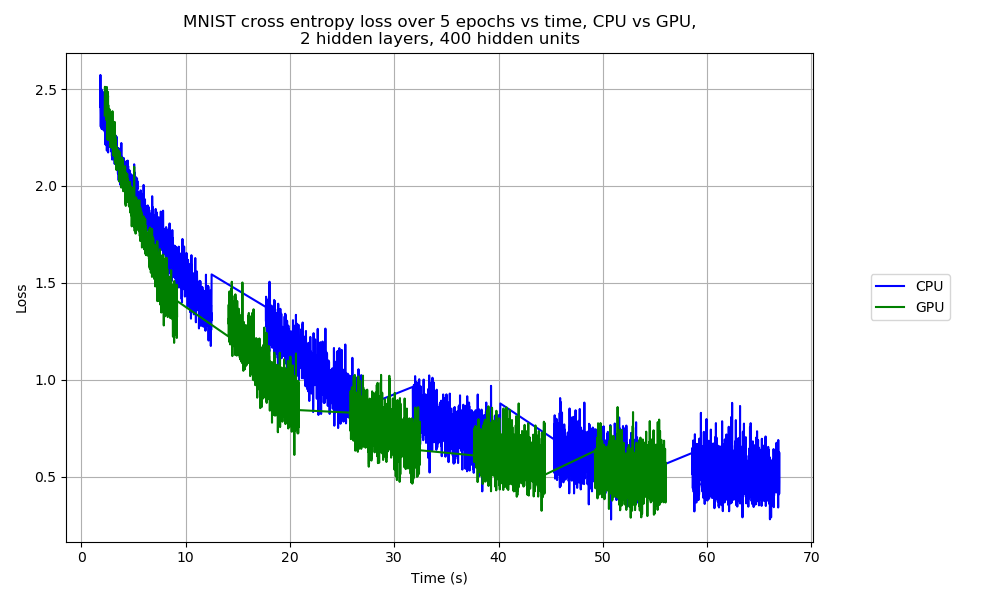
\includegraphics[width=\textwidth]{MNIST_cross_entropy_loss_over_5_epochs_vs_time,_CPU_vs_GPU,_2_hidden_layers,_400_hidden_units.png}
        \caption{Small model (2 hidden layers, 400 hidden units)}
        \label{fig:mnist small}
    \end{subfigure}
    \begin{subfigure}{0.45\textwidth}
        \centering
        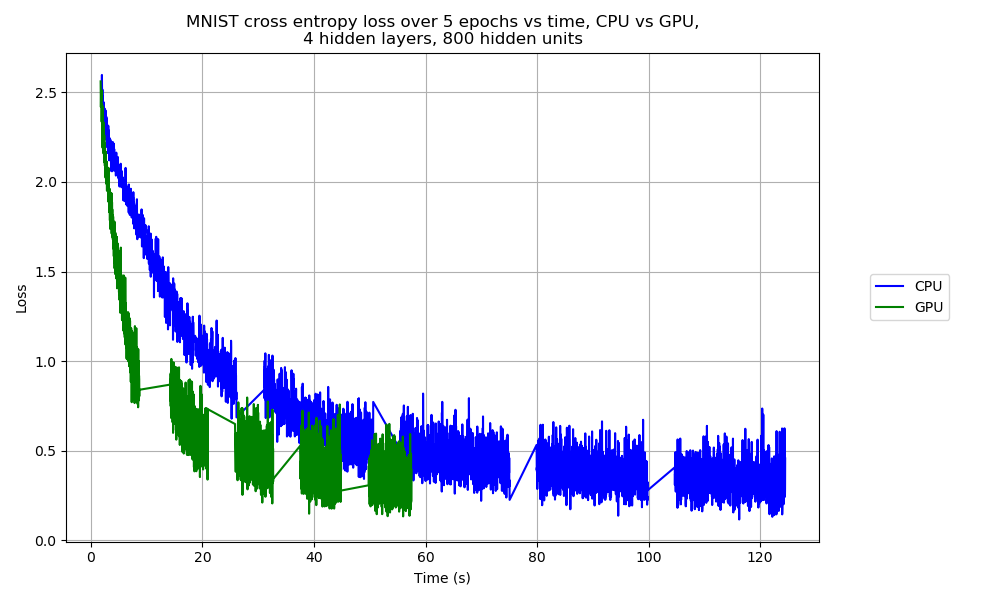
\includegraphics[width=\textwidth]{MNIST_cross_entropy_loss_over_5_epochs_vs_time,_CPU_vs_GPU,_4_hidden_layers,_800_hidden_units.png}
        \caption{Larger model (4 hidden layers, 800 hidden units)}
        \label{fig:mnist larger}
    \end{subfigure}
    \caption{Learning curves for different sized models trained on MNIST over 5 epochs, comparing training times between an Intel(R) Core(TM) i7-1065G7 CPU @ 1.30GHz and an NVIDIA GeForce MX250 GPU. Gaps in the training curves are due to evaluating test set accuracy once per epoch.}
    \label{fig:mnist cpu gpu}
\end{figure}
\begin{figure}
    \centering
    \begin{subfigure}{0.45\textwidth}
        \centering
        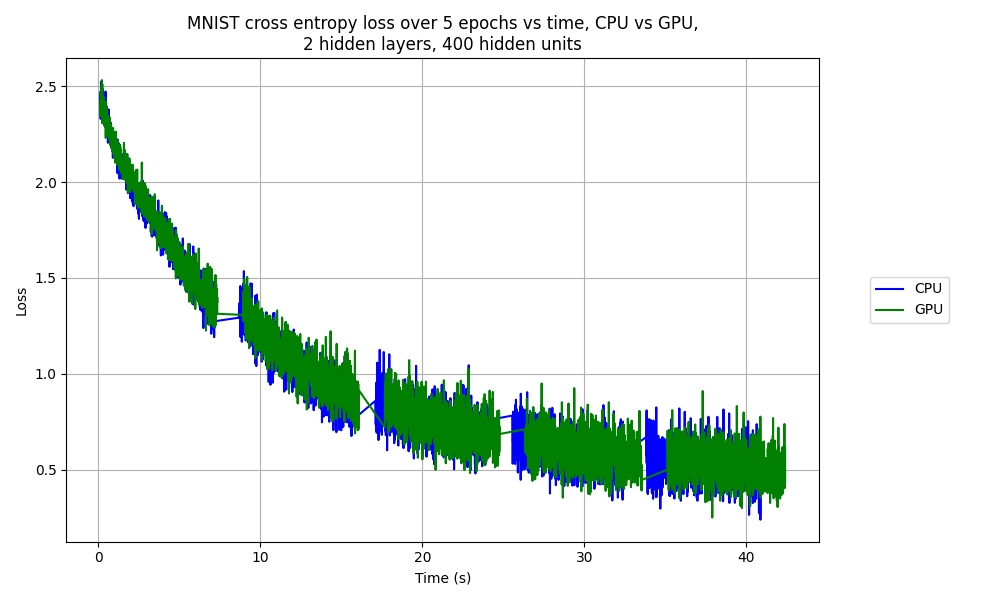
\includegraphics[width=\textwidth]{server_MNIST_cross_entropy_loss_over_5_epochs_vs_time,_CPU_vs_GPU,_2_hidden_layers,_400_hidden_units.png}
        \caption{Small model (2 hidden layers, 400 hidden units)}
        \label{fig:mnist small server}
    \end{subfigure}
    \begin{subfigure}{0.45\textwidth}
        \centering
        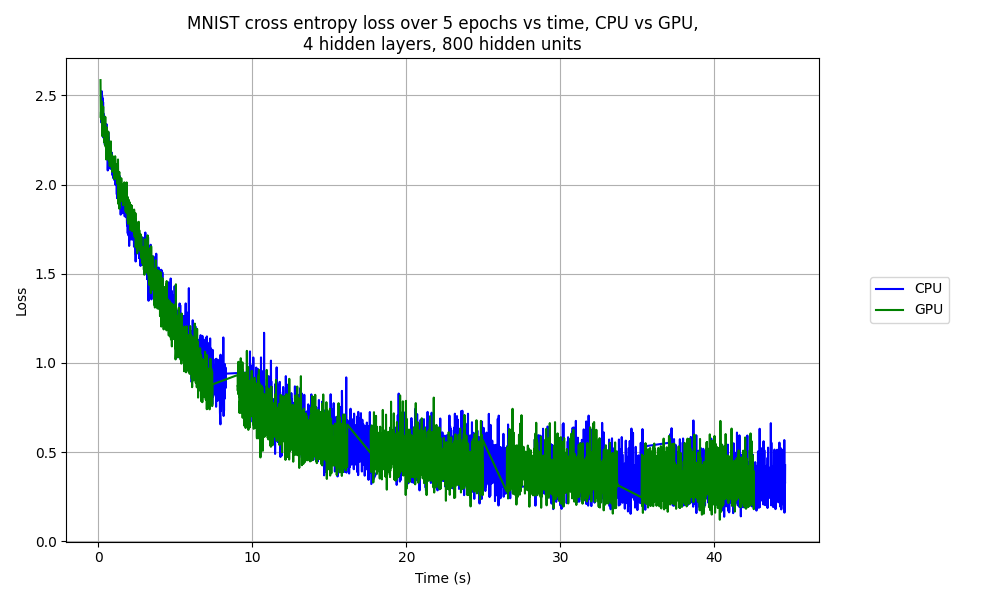
\includegraphics[width=\textwidth]{server_MNIST_cross_entropy_loss_over_5_epochs_vs_time,_CPU_vs_GPU,_4_hidden_layers,_800_hidden_units.png}
        \caption{Larger model (4 hidden layers, 800 hidden units)}
        \label{fig:mnist larger server}
    \end{subfigure}
    \caption{As for figure \ref{fig:mnist cpu gpu}, performed on a server with Intel(R) Xeon(R) Gold 5120 CPU @ 2.20GHz and NVIDIA TITAN V GPU}
    \label{fig:mnist cpu gpu server}
\end{figure}
\begin{figure}
    \centering
    \begin{subfigure}{0.45\textwidth}
        \centering
        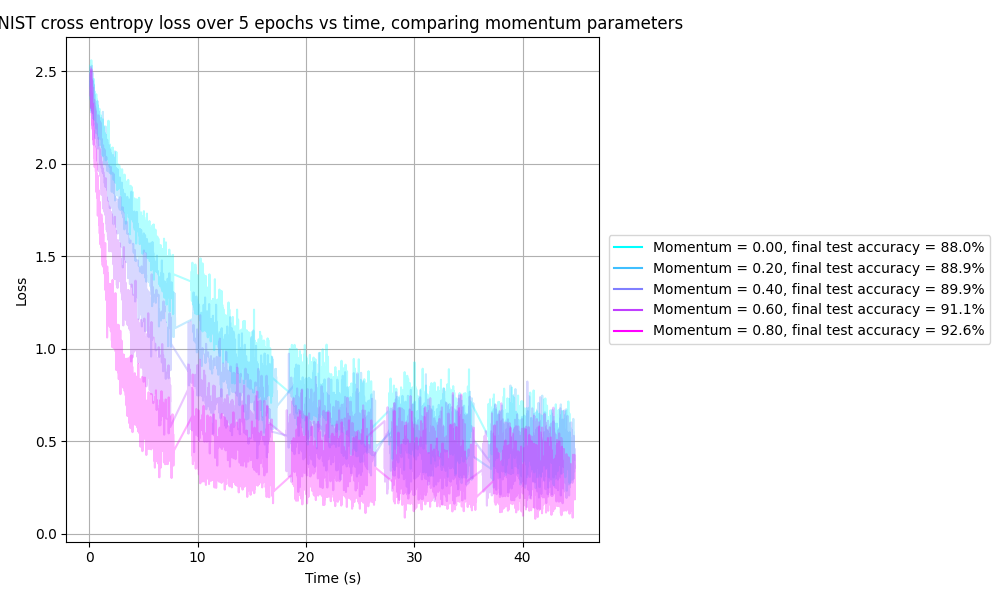
\includegraphics[width=\textwidth]{MNIST_cross_entropy_loss_over_5_epochs_vs_time,_comparing_momentum_parameters.png}
        \caption{Comparing momentum optimisation hyperparameter}
        \label{fig:mnist momentum}
    \end{subfigure}
    \begin{subfigure}{0.45\textwidth}
        \centering
        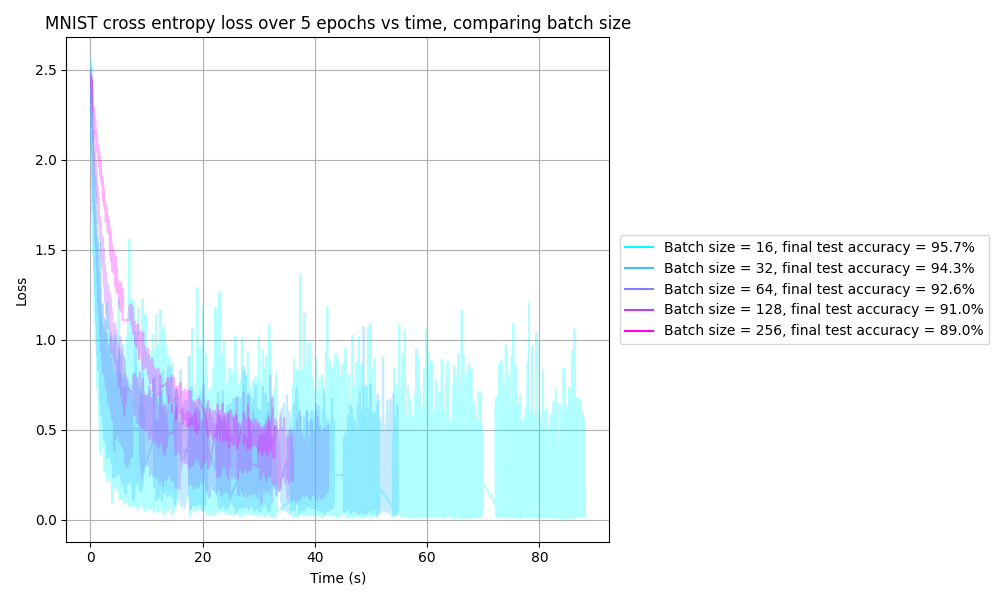
\includegraphics[width=\textwidth]{MNIST_cross_entropy_loss_over_5_epochs_vs_time,_comparing_batch_size.png}
        \caption{Comparing batch size}
        \label{fig:mnist batch size}
    \end{subfigure}
    \newline
    \begin{subfigure}{0.45\textwidth}
        \centering
        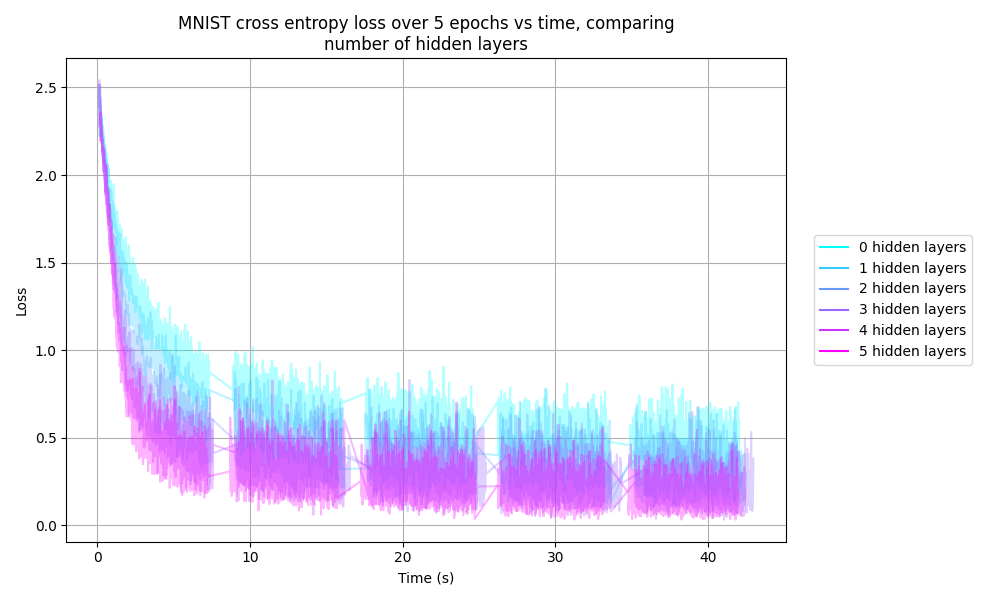
\includegraphics[width=\textwidth]{MNIST_cross_entropy_loss_over_5_epochs_vs_time,_comparing_number_of_hidden_layers.png}
        \caption{Comparing number of hidden layers}
        \label{fig:mnist num hidden layers}
    \end{subfigure}
    \begin{subfigure}{0.45\textwidth}
        \centering
        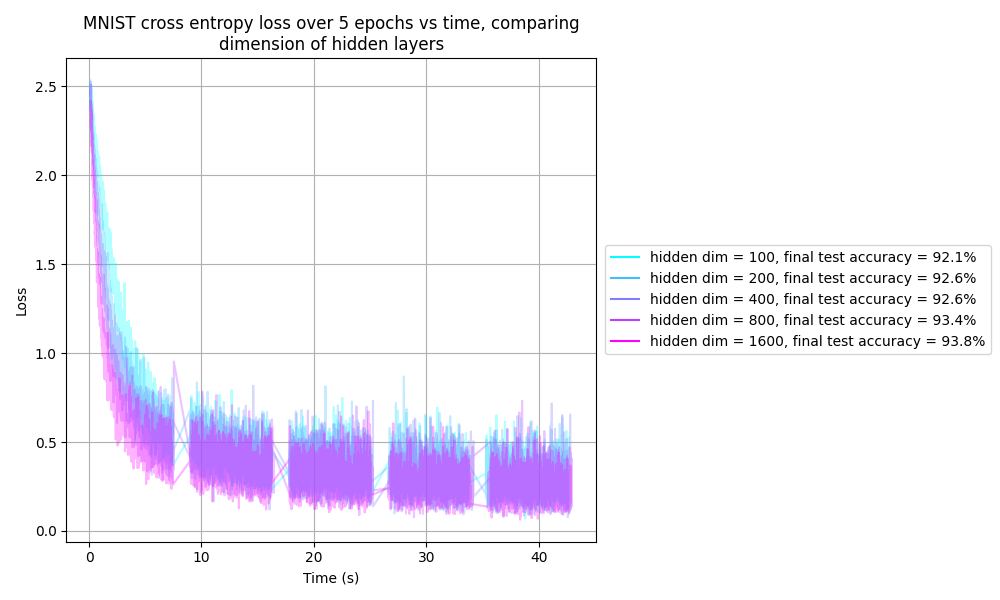
\includegraphics[width=\textwidth]{MNIST_cross_entropy_loss_over_5_epochs_vs_time,_comparing_dimension_of_hidden_layers.png}
        \caption{Comparing dimension of hidden layers}
        \label{fig:mnist hidden dimension}
    \end{subfigure}
    \newline
    \begin{subfigure}{0.45\textwidth}
        \centering
        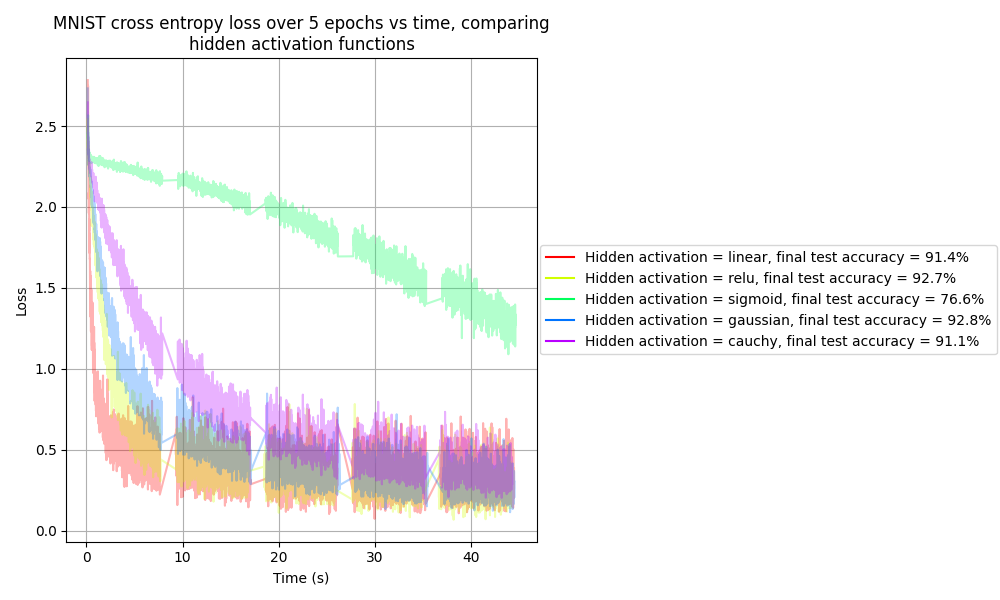
\includegraphics[width=\textwidth]{MNIST_cross_entropy_loss_over_5_epochs_vs_time,_comparing_hidden_activation_functions.png}
        \caption{Comparing hidden layer activation functions}
        \label{fig:mnist activation function}
    \end{subfigure}
    \caption{Comparing the effect of different hyperparameters on training a MLP on MNIST. Test set prediction accuracies are included in legends.}
    \label{fig:mnist parameters}
\end{figure}
\begin{figure}
    \centering
    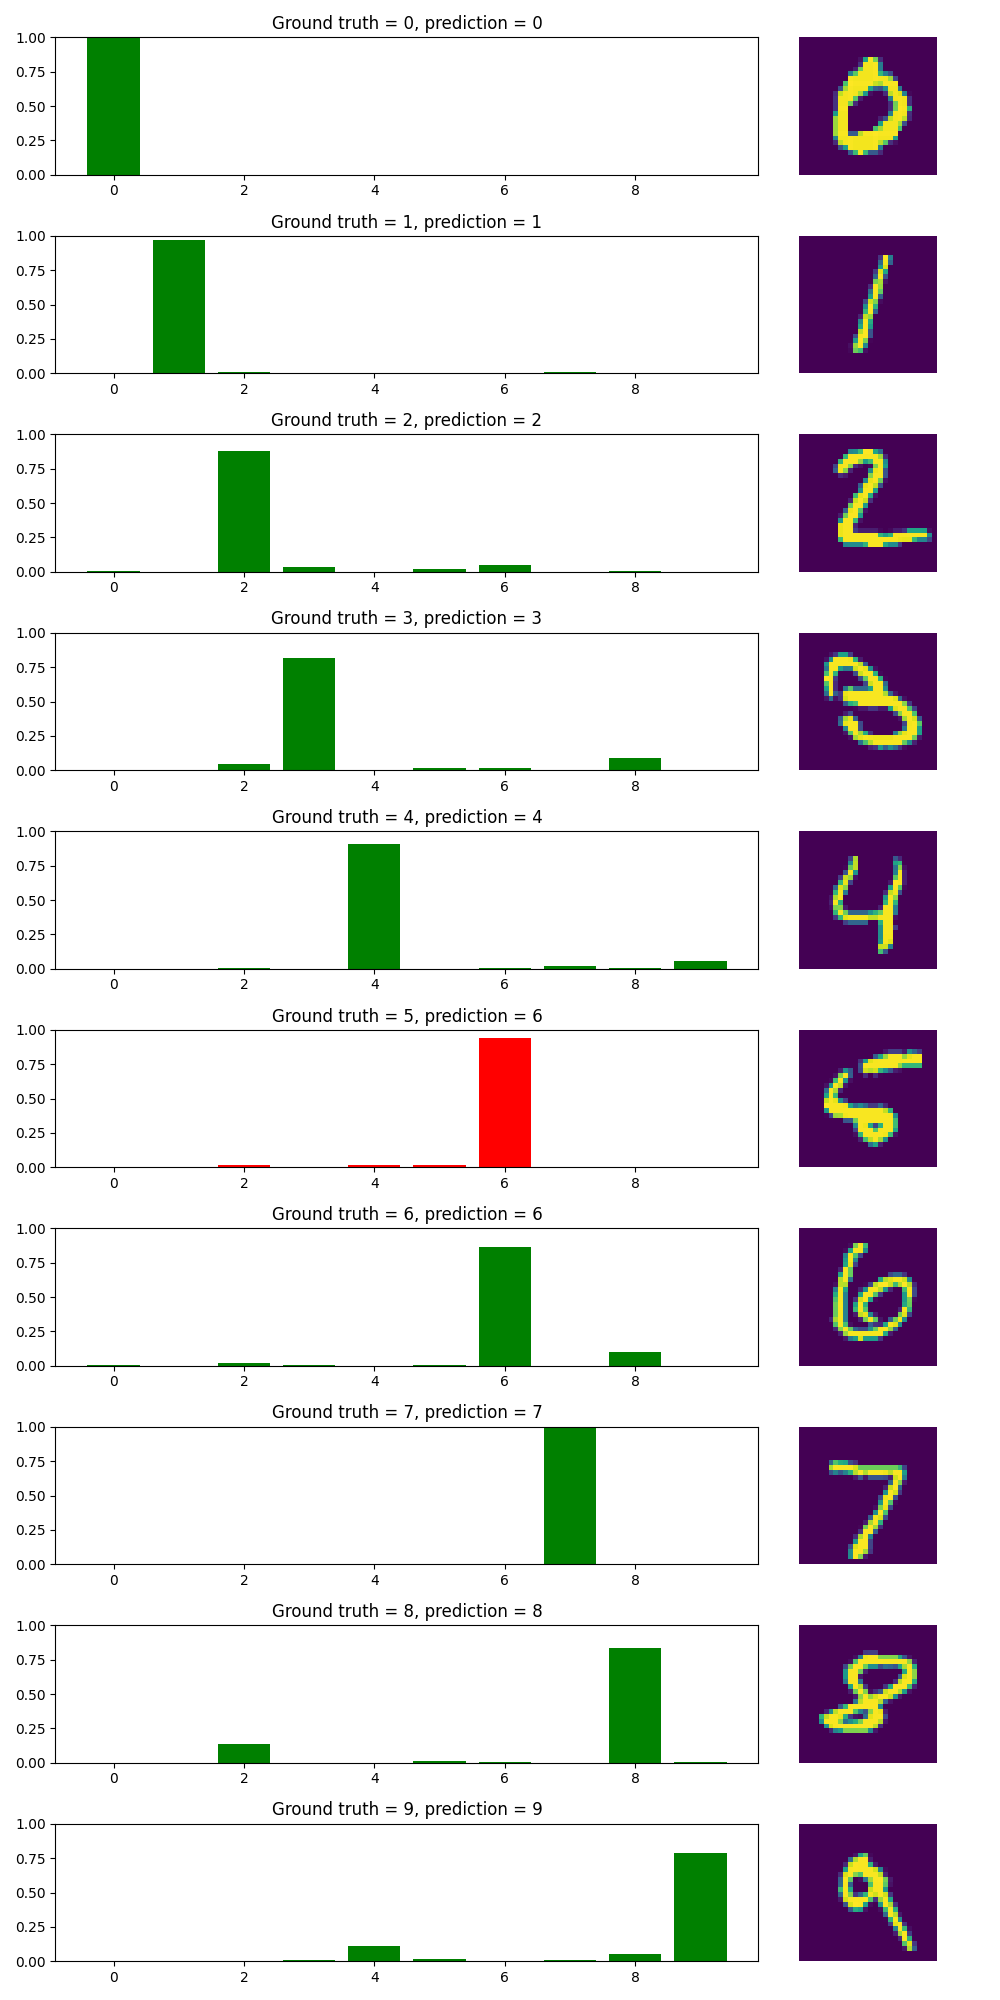
\includegraphics[width=0.6\textwidth]{Test_set_predictions.png}
    \caption{Predictions of a MLP trained on MNIST for 5 epochs on unseen examples of each digit from the test set}
    \label{fig:mnist predictions}
\end{figure}
\begin{figure}
    \centering
    \begin{subfigure}{0.6\textwidth}
        \centering
        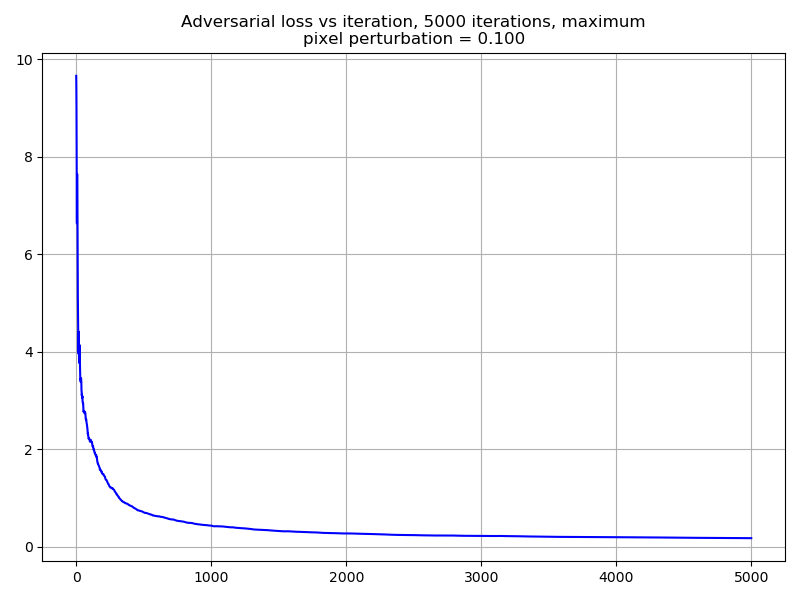
\includegraphics[width=\textwidth]{Adversarial_loss_vs_iteration,_5000_iterations,_maximum_pixel_perturbation___0.100.png}
        \caption{Adversarial loss (equation \ref{eq:adversarial problem}) vs iteration}
        \label{fig:adversarial loss}
    \end{subfigure}
    \newline
    \begin{subfigure}{\textwidth}
        \centering
        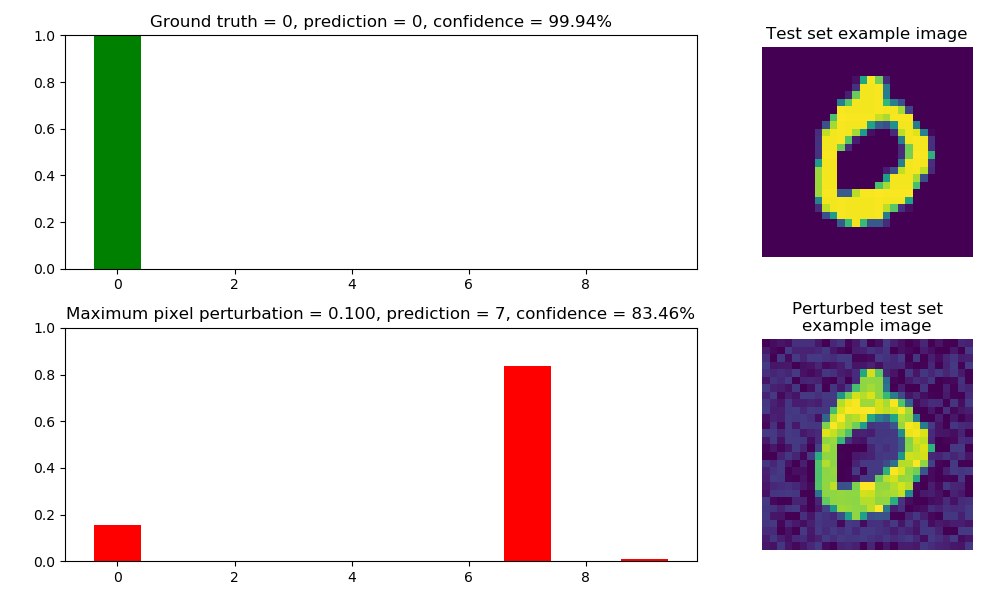
\includegraphics[width=\textwidth]{Test_set_predictions_with_adversarial_example.png}
        \caption{Trained MLP predictions for adversarial example}
        \label{fig:adversarial prediction}
    \end{subfigure}
    \caption{Training curve and predictions for an adversarial example}
    \label{fig:adversarial example}
\end{figure}
\begin{figure}
    \centering
    \begin{subfigure}{0.45\textwidth}
        \centering
        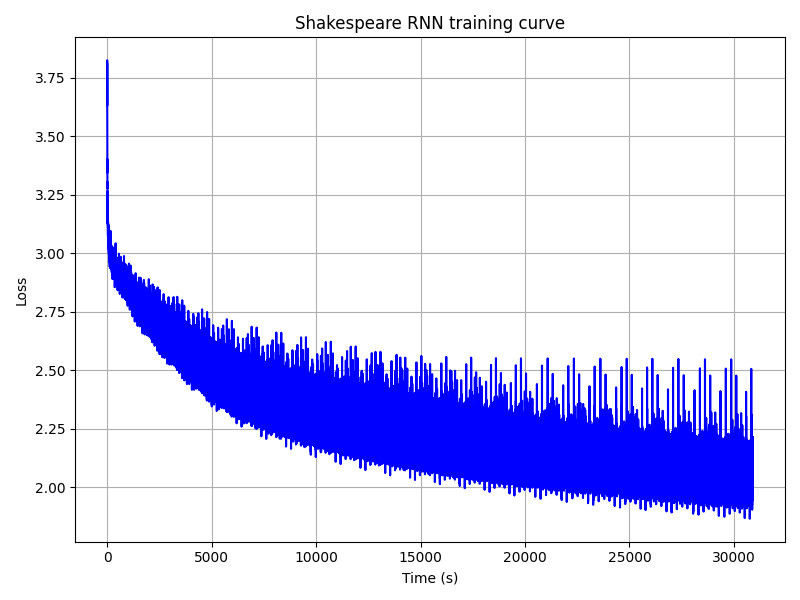
\includegraphics[width=\textwidth]{overnight_Shakespeare_RNN_training_curve.png}
        \caption{RNN}
        \label{fig:Shakespeare RNN}
    \end{subfigure}
    \begin{subfigure}{0.45\textwidth}
        \centering
        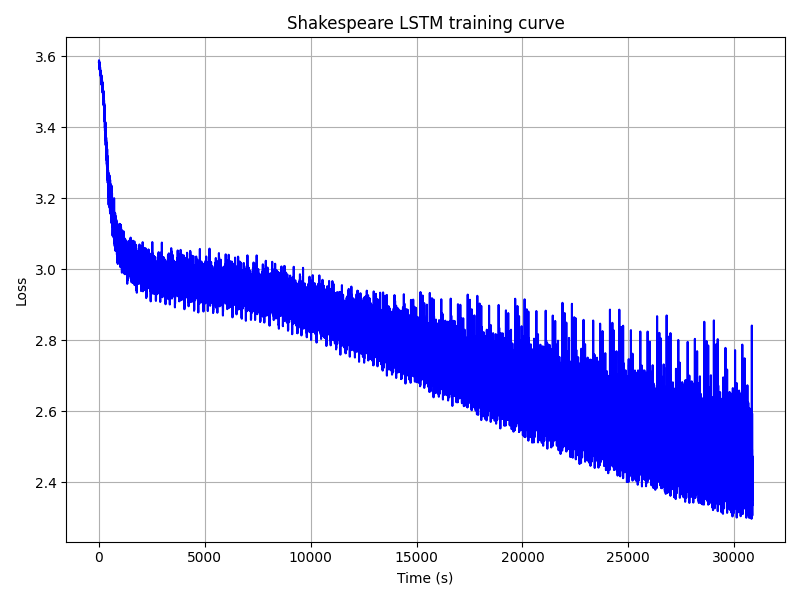
\includegraphics[width=\textwidth]{overnight_Shakespeare_LSTM_training_curve.png}
        \caption{LSTM}
        \label{fig:Shakespeare LSTM}
    \end{subfigure}
    \caption{Loss functions over time while training different sequence models on the complete works of Shakespeare, to predict the next character given a string of training data}
    \label{fig:Shakespeare}
\end{figure}

\end{document}
